\section{Human Resource Allocation}
\label{DDHR}
The first part of the project will involve a team of five specialists designing the five critical subsystems and one person designing the orbits of the swarm. The other four members will concentrate on the development of the software that will be used to assist the trade-off and verify the design. At later stages, some of the the software engineering personnel is heavily involved in designing proper algorithms for the processing of mission data, while others will be brought in to assist with detail design. 

A schematic representation of the resource allocation can be found in figure \ref{fig:DDBBHR} on page \pageref{fig:DDBBHR}.

\begin{figure}[ht!]
\begin{center}
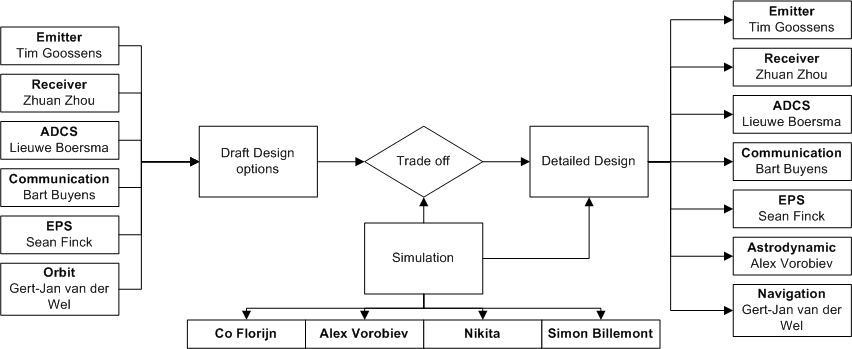
\includegraphics[width=0.9\textwidth]{chapters/img/DDBBHR.jpg}
\end{center}
\caption{Human resource allocation chart.}
\label{fig:DDBBHR}
\end{figure}

The table \ref{tab:RWD} on page \pageref{tab:RWD} gives the documentation distribution of each person on each chapter.

\newpage
\begin{center}
\begin{longtable}{|c|l|c|c|}\hline
 Chapter & Documentation                      & Author & Checked by \\\hline 
 -       & Title Page                           & Alex   & \\\hline                  
 -       & Preface                              & Co, Team& \\\hline
 -       & List of Symbol                       &\\\hline
 -       & List of Acronyms                       &\\\hline
 -       & Abstract                             & Co, Bart &\\\hline
 1       & Introduction                         &\\\hline\hline
 2       & Project Management                   &\\\hline
 2.1     & \ -Resource Allocation               & Zhuan &\\\hline
 2.2     & \ -Budget Breakdown                  & Zhuan &\\\hline
 2.3     & \ -Operations and Logistic Concept Description & GJ &\\\hline
 2.4     & \ -Project Design and Development Logic & Lieuwe &\\\hline
 2.5     & \ -Project Gantt Chart               & Lieuwe &\\\hline\hline
 3       & Mission Approach                     &\\\hline
 3.1     & \ -Function Flow Diagram             & Lieuwe, Zhuan & \\\hline
 3.2     & \ -Function Breakdown Structure      & Lieuwe, Zhuan &\\\hline
 3.3     & \ -H/W Block Diagram                 & Lieuwe, &\\\hline
 3.4     & \ -S/W Block Diagram                 & Nikita &\\\hline
 3.5     & \ -Electrical Block Diagram          & Sean &\\\hline
 3.6     & \ -Data Handling Block Diagram       & GJ &\\\hline
 3.7     & \ -Communication Block Diagram       & Bart &\\\hline
 4       & Risk Management                      & Tim, Zhuan & \\\hline\hline
 5       & Launch and Astrodynamic Characteristics & Alex &\\\hline
 5.1     & \ -Launch Segment                    & Alex &\\\hline
 5.2     & \ -Space Segment                     & Alex &\\\hline
 5.3     & \ -Space Environment and Shielding   & Alex &\\\hline\hline
 6       & Emitter                              &&\\\hline
 6.1     & \ -OEP                               & Tim &\\\hline
 6.1.1   & \ \ -Principle of Diode Laser       & Tim &\\\hline
 6.1.2   & \ \ -Diode Pumped Laser Configuration & Tim &\\\hline
 6.1.3   & \ \ -Optical Characteristics        & Tim &\\\hline
 6.1.4   & \ \ -Diffraction                    & Tim &\\\hline  
 6.1.5   & \ \ -Thermal Control                & Tim, Lieuwe &\\\hline
 6.1.6   & \ \ -Laser Life Time Expectancy     & Tim &\\\hline
 6.1.7   & \ \ -Laser Focus Calculation        & Zhuan &\\\hline
 6.2     & \ -Navigation                        & GJ &\\\hline
 6.3     & \ -Communication                     & Bart &\\\hline
 6.4     & \ -ADCS                              & Lieuwe &\\\hline
 6.5     & \ -EPS                               & Sean &\\\hline
 6.6     & \ -Summary                           &&\\\hline\hline
 7       & Receiver                             &&\\\hline
 7.1     & \ -ORP                               & Zhuan &\\\hline
 7.1.2   & \ \ -SPAD Research                  & Tim, Zhuan &\\\hline
 7.1.3   & \ \ -Prism Design                   & Zhuan &\\\hline
 7.1.4   & \ \ -Summary                        & Zhuan &\\\hline
 7.1.5   & \ \ -Payload Cost Estimation        & Tim, Zhuan &\\\hline
 7.1.6   & \ -Navigation                        & GJ &\\\hline
 7.2     & \ -Communication                     & Bart &\\\hline
 7.3     & \ -ADCS                              & Lieuwe &\\\hline
 7.4     & \ -EPS                               & Sean &\\\hline
 7.5     & \ -Summary                           &&\\\hline\hline
 8       & Data Validation                      & Simon, Co, Nikita &\\\hline
 8.1     & \ -Software Tool Internals           & Simon, Co, Nikita &\\\hline
 8.2     & \ -Validation Results                & Simon, Co, Nikita &\\\hline
 9       & Sustainable Development Strategy     &&\\\hline
 10      & Compliance Matrix                    &&\\\hline\hline
 11      & Conclusion and Recommendations         &&\\\hline\hline
 -       & Others                               &&\\\hline
 -       & \ -Catia Drawing                     & Lieuwe &\\\hline
 -       & \ -Latex Compile                     & Zhuan &\\\hline

\caption{Report writing distribution.}
\label{tab:RWD}
\end{longtable}
\end{center}

%%%%%%%%%%%%%%%%%%%%%%%%%%%%%%%%%%%%%%%%%%%%%%%%%%%%%%%%%%%%%%%%%%%%%%%%%%%%%%%%%%%%%%%%%%%%%
\section{Mass Budget Breakdown}
\label{DDMBB}
The table \ref{tab:MB} on page \pageref{tab:MB} indicates mass budget breakdown for emitter and receiver satellites. The table is mainly divided into two parts. The first part gives each subsystem mass of emitter and receiver satellites in both kilograms and percentage of total dry mass. Meanwhile, the second part includes the mass of propellants and then also gives the total mass when the satellites are in their orbit. The deviation of all numbers in the table can be found in each corresponding chapter of the subsystem.

\begin{table}[ht!]
\centering
\begin{tabular}{|l|c|c|c|c|}
\hline
 & \multicolumn{2}{|c|}{Emitter} & \multicolumn{2}{|c|}{Receiver} \\\hline
 Subsystem        & $M [kg]$ & \%$M_{dry}$ & $M [kg]$ & \%$M_{dry}$ \\\hline\hline
 Communication    & 10.66    & 21          & 3        & 22.2 \\\hline
 Navigation       & 0.25     & 0.5         & 0.25     & 1.85 \\\hline
 OEP              & 15       & 29.8        & -        & - \\\hline
 ORP              & 0.22     & 0.4         & 0.22     & 1.63 \\\hline
 EPS              & 5.8      & 11.5        & 3.6      & 26.6 \\\hline
 ADCS             & 2        & 4           & 2        & 14.8 \\\hline
 Thermal          & 1.48     & 3           & 0.3      & 2.22 \\\hline
 Structure        & 12.35    & 24.5        & 2.45     & 18.12 \\\hline
 Propulsion(tank) & 1        & 2           & 0.75     & 5.55 \\\hline
 Thruster         & 0.65     & 1.3         & 0.15     & 1.11 \\\hline
 Shielding        & 1        & 2           & 0.8      & 5.92 \\\hline\hline
 $M_{dry}$        & 50.41    & 100         & 13.52    & 100 \\\hline
 $M_{propellant}$ & 4        & -           & 1.5      & - \\\hline
 $M_{Loaded}$     & 54.41    & -           & 15.02    & - \\\hline
 $M_{Orbit}$      & 53.1     & -           & 14.92    & - \\\hline
\end{tabular}
\caption{Mass Budget Breakdown of the emitter and a representative receiver satellites.}
\label{tab:MB}
\end{table}

%%%%%%%%%%%%%%%%%%%%%%%%%%%%%%%%%%%%%%%%%%%%%%%%%%%%%%%%%%%%%%%%%%%%%%%%%%%%%%%%%%%%%%%%%%%%%
\section{Cost Budget Breakdown}
\label{DDCB}
Figure \ref{fig:lifecycle} on page \pageref{fig:lifecycle} shows a typical life-cycle for a space mission. The \ac{RDTE} stage includes the planning, development and testing of all prototypes and qualification units, but does not include the technology development for different subsystems. In the case of the laser swarm this is largely dependent on the single emitter and one receiver unit. This stage is also mostly consistent of non-recurring costs. The production stage consists of actual manufacture of the physical satellites. The cost estimation in this stage is based on the \ac{TFU}. This is done because it is assumed that the first unit (in the case of the Laser Swarm, that would be the emitter and one receiver) would be the most expensive to produce. The rest of the swarm constellation satellite costs are calculated by taking a theoretical learning curve \cite{larson}. 

\begin{figure}[ht!]
\centering
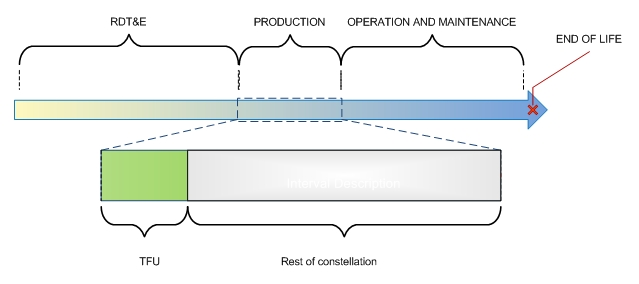
\includegraphics[scale = 0.8]{chapters/img/lifetime.jpg}
\caption{Satellite Life-Cycle}
\label{fig:lifecycle}
\end{figure}

The table \ref{tab:CB} on page \pageref{tab:CB} gives the cost breakdown of both theoretical first unit cost for either emitter or receiver satellite and also the swarm of 9 satellites including all the wraps.

\begin{table}[ht!]
\centering
\begin{tabular}{l|c|c|c|c|c|c|}
\cline{2-7}
  & \multicolumn{4}{|c|}{Unit Cost} & \multicolumn{2}{|c|}{\multirow{2}{*}{Swarm (9 satellites)}} \\\cline{2-5}
  
  & \multicolumn{2}{|c|}{Emitter satellite} & \multicolumn{2}{|c|}{receiver satellite} & \multicolumn{2}{|c|}{ } \\\hline
  
 \multicolumn{1}{|c|}{Subsystem} & Cost [k\$] & \%Subtotal & Cost [k\$] & \%Subtotal & Cost [k\$] & \%Subtotal \\\hline
                                     %  cost [k$] %Total 
 \multicolumn{1}{|l|}{\textbf{Payload}}       & 8215.96 & 41.5 & 4048.74 & 46.58 & 8660 & 25.3 \\\hline
 \multicolumn{7}{|l|}{\textbf{Bus Total}}     \\\hline
 \multicolumn{1}{|l|}{Structure}     & 1920.38 & 9.7 & 843.2 & 9.7 & 3322.33 & 9.7 \\\hline
 \multicolumn{1}{|l|}{Thermal}       & 217.776 & 1.1 & 95.62 & 1.1 & 376.76 & 1.1 \\\hline
 \multicolumn{1}{|l|}{EPS}           & 541 & 2.7 & 266 & 3.06 & 1193.694 & 3.49 \\\hline
 \multicolumn{1}{|l|}{Navigation}    & 25   & 0.13 & 25 & 0.29 & 191.235 & 0.558 \\\hline
 \multicolumn{1}{|l|}{Communication} & 2940 & 14.9 & 612.5 & 7.05 & 7141.14 & 20.85 \\\hline
 \multicolumn{1}{|l|}{\acs{ADCS}}    & 199.093 & 1 & 175.914 & 2.02 & 1405.687 & 4.1 \\\hline
 \multicolumn{1}{|l|}{Tank}          & 0.713 & 0.0036 & 0.428 & 0.0049 & 3.649 & 0.011 \\\hline
 \multicolumn{1}{|l|}{Thruster}      & 570.64  & 2.88 & 356.65  & 4.1 & 3016.9 & 8.8 \\\hline
 \multicolumn{7}{|l|}{\textbf{Wraps}}     \\\hline
 \multicolumn{1}{|l|}{\acs{IAT}}     & 1445.24 & 7.3 & 634.58 & 7.3 & 2500.34 & 7.3 \\\hline
 \multicolumn{1}{|l|}{Program Level} & 2395.53 & 12.1 & 1051.84 & 12.1 & 4144.36 & 12.1 \\\hline
 \multicolumn{1}{|l|}{\acs{GSE}}     & 692.92 & 3.5 & 304.25 & 3.5 & 1198.78 & 3.5 \\\hline
 \multicolumn{1}{|l|}{\acs{LOOS}}    & 633.53 & 3.2 & 278.17 & 3.2 & 1096.03 & 3.2 \\\hline
 \multicolumn{1}{|l|}{Subtotal}      & 19797.79 & 100 & 8692.92 & 100 & 34250.88 & 100 \\\hline
 \multicolumn{1}{|l|}{Launch}        & - & - & - & - & 18534.25 & - \\\hline\hline\hline
 \multicolumn{1}{|l|}{\textbf{Total}}         & - & - & - & - & 52785.13 & - \\\hline
 \multicolumn{1}{|l|}{\textbf{Total (FY00)}}  & - & - & - & - & 43089.90 & - \\\hline
 
\end{tabular}
\caption{Cost Budget Breakdown.}
\label{tab:CB}
\end{table}